% !TEX program = lualatex
% !TEX encoding = UTF-8 Unicode
\documentclass[12pt,xcolor={rgb},t]{beamer}

\usetheme{dirichlet}

\usepackage{color}
\usepackage{arev}
\usepackage{graphicx}
\usepackage{pdfpages}
\usepackage{listings}
\usepackage[english]{babel}
\usepackage{hyperref}
\usepackage{pgfplots}
\usepackage{tikz}
\usepackage{ifthen}
\usepackage{MnSymbol}
\usetikzlibrary{positioning}
\usetikzlibrary{graphs,graphs.standard,quotes}
\usetikzlibrary{patterns}
\usepackage{pgfplotstable}
\usepackage{filecontents}

\usepackage{amsmath,amsfonts,amssymb}

\usepackage{xcolor}
\usepackage{hyperref}

\hypersetup{colorlinks=false,urlcolor=cyan}

\begin{document}

\title{MD-Bench}
\author{Maximilian Gaul}
\institute{MuCoSim Seminar}

\begin{frame}[plain]
\titlepage
\end{frame}

\section{Preliminary}

\definecolor{brightcerulean}{rgb}{0.11, 0.67, 0.84}

\begin{frame}{About}

    \begin{itemize}
        \item MD-Bench is a molecular dynamics application which calculates the intersections among particles and how these affect motion
        \item Simulation system consists of:
        \begin{itemize}
            \item Number of atoms, each having an initial state and velocity
            \item Boundary conditions
        \end{itemize}
        \item The force of each atom is a sum of its interactions with neighboring atoms
    \end{itemize}

\end{frame}

\begin{frame}[fragile]{Force modeling}

    \begin{itemize}
        \item In MD-Bench, the Lennard-Jones potential is used for calculating the forces between pairs of particles \cite{MACHADO2021101425}
        \begin{itemize}
            \item In our case, particles are electronically neutral atoms
        \end{itemize}
        \item This function models repulsive as well as attractive interactions
        $$V_{LJ}(r) = 4\epsilon \left[\left( \frac{\sigma}{r} \right)^{12} - \left( \frac{\sigma}{r} \right)^6 \right]$$
    \end{itemize}

\end{frame}

\begin{frame}[fragile]{The Lennard-Jones potential I}
    
    $$V_{LJ}(r) = 4\epsilon \left[\left( \frac{\sigma}{r} \right)^{12} - \left( \frac{\sigma}{r} \right)^6 \right]$$
    \begin{itemize}
        \item Where
        \begin{itemize}
            \item \textbf{r} is the distance between two interacting atoms
            \item \textbf{$\epsilon$} is the dispersion energy
            \item \textbf{$\sigma$} is the distance at which the potential \textbf{V} is equal to zero
        \end{itemize}
    \end{itemize}

\end{frame}

\begin{frame}[fragile]{The Lennard-Jones potential II}

    \begin{itemize}
        \item Behavior of the Lennard-Jones potential with increasing distance \textbf{r} in \textbf{Å} (Ångström)
        \vspace{1em}
        \begin{figure}[H]
            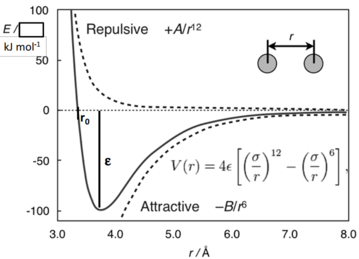
\includegraphics[width=6cm]{Images/Lennard_Jones_potential_function.png}
            \caption{ Lennard Jones Potential }
        \end{figure}
    \end{itemize}
    
\end{frame}

\begin{frame}[fragile]{The Lennard-Jones potential III}

    \begin{itemize}
        \item The Lennard-Jones potential is a simplified model but still describes the essential aspects of particle dynamics
        \item We observe that particles
        \begin{itemize}
            \item repel each other at close distance
            \item attract each other at medium distances and have
            \item close to zero interaction at  large distances
        \end{itemize}
    \end{itemize}
    
\end{frame}

\section{Testsystem}

\begin{frame}[fragile]{Cluster}

    \begin{itemize}
        \item Host/Clustername: tinyGPU.tg086
        \item Cluster Info
        \begin{itemize}
            \item https://hpc.fau.de/systems-services/systems-documentation-instructions/clusters/tinygpu-cluster/
        \end{itemize}
        \item CPU type: 2x Intel Xeon Gold 6226R @2.9 GHz = 32 cores with optional SMT
        \item GPU type: 8x NVIDIA Geforce RTX3080
        \item Memory capacity: 384 GB RAM
        \item Software Environment:
        \begin{itemize}
            \item Compiler: NVIDIA NVCC Build cuda\_11.2.r11.2
            \item Operating System: Ubuntu 20.04.3 LTS
        \end{itemize}
    \end{itemize}

\end{frame}

\section{MD-Bench}

\begin{frame}[fragile]{Force calculation I}

    \lstset{language=Python,
        basicstyle=\ttfamily,
        keywordstyle=\color{brightcerulean}\ttfamily,
        stringstyle=\color{red}\ttfamily,
        commentstyle=\color{green}\ttfamily,
        morecomment=[l][\color{magenta}]{\#}
    }
    \begin{itemize}
        \item Calculation of the Lennard-Jones potential is done for pairs of atoms (pseudocode):
\begin{lstlisting}[basicstyle=\footnotesize, language=Python]
for atom in atoms:
    neighbors = neighbor.neighbors[atom]
    force = 0.0
    for neighbor in neighbors:
        radius = calc_radius(...)
        if radius < close_enough:
            force += calc_force(...)
    forces[atom] += force
\end{lstlisting}
    \end{itemize}
    
\end{frame}

\begin{frame}[fragile]{Force calculation II}

    \begin{itemize}
        \item It is time consuming and unnecessary to calculate the force for \textit{every} pair of atoms if they are so far apart that the force is close to 0 anyways
        \begin{figure}[H]
            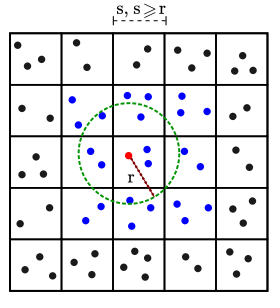
\includegraphics[width=4cm]{Images/Neighbor_list_MD_Bench.png}
            \caption{ Neighbor list \cite{MACHADO2021101425} }
        \end{figure}
    \end{itemize}

\end{frame}

\begin{frame}[fragile]{Configuration}

    \lstset{prebreak=\raisebox{0ex}[0ex][0ex]
        {\ensuremath{\rhookswarrow}}}
    \lstset{postbreak=\raisebox{0ex}[0ex][0ex]
        {\ensuremath{\rcurvearrowse\space}}}
    \lstset{breaklines=true, breakatwhitespace=true}

    \begin{itemize}
        \item Clone the repository
\begin{lstlisting}[basicstyle=\footnotesize, language=Bash, linewidth=10cm]
foo@bar:~$ git clone https://github.com/RRZE-HPC/MD-Bench.git
foo@bar:~$ cd MD-Bench
foo@bar:~/MD-Bench$ git checkout mucosim_cuda
\end{lstlisting}
        \item Load modules
\begin{lstlisting}[basicstyle=\footnotesize, language=Bash]
foo@bar:~/MD-Bench$ module load cuda likwid
\end{lstlisting}
        \item Change
        \begin{itemize}
            \item \lstinline{TAG} variable in \lstinline{config.mk} to \lstinline{TAG ?= NVCC}
            \item Compiler flags in \lstinline{include_NVCC.mk}
        \end{itemize}
    \end{itemize}

\end{frame}

\begin{frame}[fragile]{Run Software}
    
    \lstset{prebreak=\raisebox{0ex}[0ex][0ex]
        {\ensuremath{\rhookswarrow}}}
    \lstset{postbreak=\raisebox{0ex}[0ex][0ex]
        {\ensuremath{\rcurvearrowse\space}}}
    \lstset{breaklines=true, breakatwhitespace=true}

    \begin{itemize}
        \item Compile and execute
\begin{lstlisting}[basicstyle=\footnotesize, language=Bash, linewidth=10cm]
foo@bar:~/MD-Bench$ make
foo@bar:~/MD-Bench$ ./MDBench-NVCC
\end{lstlisting}
        \item MD-Bench will output temperature and pressure data as well as performance in million atom updates per second
        \item Modify number of runs with argument \lstinline{-n <nmbr>}
    \end{itemize}

\end{frame}

\begin{frame}[fragile]{Program Output}
    
    \lstset{prebreak=\raisebox{0ex}[0ex][0ex]
        {\ensuremath{\rhookswarrow}}}
    \lstset{postbreak=\raisebox{0ex}[0ex][0ex]
        {\ensuremath{\rcurvearrowse\space}}}
    \lstset{breaklines=true, breakatwhitespace=true}

    \begin{itemize}
        \item With unmodified parameters
\begin{lstlisting}[basicstyle=\footnotesize, linewidth=10cm]
step    temp            pressure
0       1.440000e+00    1.215639e+00
100     8.200895e-01    6.923143e-01
200     7.961495e-01    6.721043e-01
---------------------------------------------------
Force field: lj
Data layout for positions: AoS
Using double precision floating point.
---------------------------------------------------
System: 131072 atoms 47265 ghost atoms, Steps: 200
TOTAL 6.83s FORCE 0.73s NEIGH 3.07s REST 3.04s
---------------------------------------------------
Performance: 3.84 million atom updates per second
\end{lstlisting}
    \end{itemize}

\end{frame}

\section{Scaling runs}

\begin{frame}[fragile]{CUDA I}
    
    \begin{itemize}
        \item CUDA programming model
        \begin{itemize}
            \item Basic execution size is a \textit{thread} which is executed by one CUDA core
            \item Threads are grouped together as \textit{blocks}, these are executed by
            streaming multiprocessors (\textit{SM})
            \item Resources on an SM are allocated on a \textit{warp}-size level (32 threads)
            \item Warps are dispatched to execution units of GPU
        \end{itemize}
    \end{itemize}

\end{frame}

\begin{frame}[fragile]{CUDA II}
    
    \begin{itemize}
        \item \lstinline{src/force.c} was refactored to support CUDA kernel functions and distribution on multiple Threads of a GPU
        \item Force-calculation is parallelized on an atom-level
        \item Each atom computes the force for every other atom in its neighbor list (around 100)
    \end{itemize}

\end{frame}

\begin{frame}[fragile]{Scaling threads I}
    
    \lstset{language=Python,
        basicstyle=\ttfamily,
        keywordstyle=\color{brightcerulean}\ttfamily,
        stringstyle=\color{red}\ttfamily,
        commentstyle=\color{green}\ttfamily,
        morecomment=[l][\color{magenta}]{\#}
    }
    \lstset{prebreak=\raisebox{0ex}[0ex][0ex]
        {\ensuremath{\rhookswarrow}}}
    \lstset{postbreak=\raisebox{0ex}[0ex][0ex]
        {\ensuremath{\rcurvearrowse\space}}}
    \lstset{breaklines=true, breakatwhitespace=true}

    \begin{itemize}
        \item Default number of atoms: \textit{131072}
        \item Around $10^7$ force computations per run
        \item Number of blocks is calculated by (\lstinline{num_threads} is fixed):
\begin{lstlisting}[basicstyle=\footnotesize, language=Python]
blocks = ceil( 131072 / num_threads )
\end{lstlisting}
        \item Run on cluster with one GPU:
\begin{lstlisting}[basicstyle=\footnotesize, language=Bash, linewidth=10cm]
foo@bar:~/MD-Bench$ srun.tinygpu -N 1 -n 1 --gres=gpu:1 --pty /bin/bash -l
foo@bar:~/MD-Bench$ NUM_THREADS=X ./MD-Bench-NVCC -n 50
\end{lstlisting}
    \end{itemize}

\end{frame}

\begin{frame}[fragile]{Scaling threads II}

    \begin{itemize}
        \item As resources are allocated on a warp-size level, we expect to have highest performance for 32 threads per block
        \begin{figure}[!H]
            \centering
            \begin{tikzpicture}[scale=0.675]
                \begin{axis}[
                    xlabel=$\text{Threads per Block}$,
                    ylabel=$\text{Atom updates per s}$,
                    xmin=1, xmax=32,
                    ymin=0, ymax=8e6,
                    legend style={fill=none,draw=white}
                ]
            
                \addplot [magenta,mark=*,smooth] table [x=threads,y=updates,col sep=comma] {Resources/gpu.csv};
                \addlegendentry{Data}
                \end{axis}
            \end{tikzpicture}
        \end{figure}
    \end{itemize}
    
\end{frame}

\begin{frame}[fragile]{Scaling threads III}

    \lstset{prebreak=\raisebox{0ex}[0ex][0ex]
        {\ensuremath{\rhookswarrow}}}
    \lstset{postbreak=\raisebox{0ex}[0ex][0ex]
        {\ensuremath{\rcurvearrowse\space}}}
    \lstset{breaklines=true, breakatwhitespace=true}

    \begin{itemize}
        \item Performance improvement stagnates
        \item But how does the CPU perform?
\begin{lstlisting}[basicstyle=\footnotesize, language=Bash, linewidth=10cm]
foo@bar:~/MD-Bench$ srun.tinyfat --ntasks=1 --cpus-per-task=32 --pty /bin/bash -l
\end{lstlisting}
        \begin{figure}[!H]
            \centering
            \begin{tikzpicture}[scale=0.625]
                \begin{axis}[
                    xlabel=$\text{OMP Num Threads}$,
                    ylabel=$\text{Atom updates per s}$,
                    xmin=1, xmax=32,
                    ymin=0, ymax=8e6,
                    legend style={fill=none,draw=white}
                ]
            
                \addplot [magenta,mark=*,smooth] table [x=threads,y=updates,col sep=comma] {Resources/cpu.csv};
                \addlegendentry{Data}
                \end{axis}
            \end{tikzpicture}
        \end{figure}
    \end{itemize}
    
\end{frame}

\section{Measurements}

\begin{frame}[fragile]{Memory Bandwidth I}

    \lstset{prebreak=\raisebox{0ex}[0ex][0ex]
        {\ensuremath{\rhookswarrow}}}
    \lstset{postbreak=\raisebox{0ex}[0ex][0ex]
        {\ensuremath{\rcurvearrowse\space}}}
    \lstset{breaklines=true, breakatwhitespace=true}

    \begin{itemize}
        \item Using the NVIDIA \textit{nvprof} profiling tool via
\begin{lstlisting}[basicstyle=\footnotesize, language=Bash, linewidth=10cm]
foo@bar:~/MD-Bench$ nvprof --print-gpu-trace ./MDBench-NVCC -n 50
\end{lstlisting}
        enables detailed metrics on memory throughput
        \vspace{1em}
        \begin{figure}[!H]
            \centering
            \scalebox{.45}{
                \pgfplotstabletypeset[
                    col sep=comma,
                    string type,
                    columns={Duration,Size,Throughput,SrcMemType,DstMemType,Name},
                    assign column name/.style={/pgfplots/table/column name={\large{\textbf{#1}}}}
                ] {Resources/nvprof.csv}
            }
        \end{figure}
    \end{itemize}

\end{frame}

\begin{frame}[fragile]{Memory Bandwith II}

    \begin{itemize}
        \item Together with analysis of the output profile in NVIDIA Nsight Systems:
        \vspace{1em}
        \begin{figure}[H]
            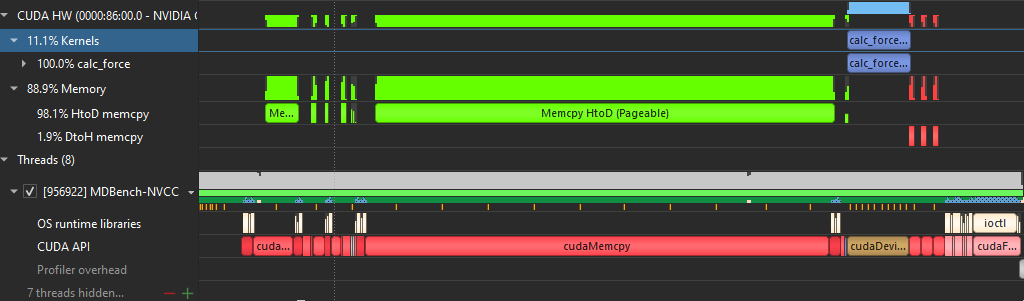
\includegraphics[width=9cm]{Images/nvidia_nsight_systems_perf_analysis.png}
            \caption{ NVIDIA Nsight Systems }
        \end{figure}
    \end{itemize}
    
\end{frame}

\begin{frame}[fragile]{Memory Bandwith III}

    \lstset{prebreak=\raisebox{0ex}[0ex][0ex]
        {\ensuremath{\rhookswarrow}}}
    \lstset{postbreak=\raisebox{0ex}[0ex][0ex]
        {\ensuremath{\rcurvearrowse\space}}}
    \lstset{breaklines=true, breakatwhitespace=true}

    \begin{itemize}
        \item and the roofline model from
\begin{lstlisting}[basicstyle=\footnotesize, linewidth=10cm]
foo@bar:~/MD-Bench$ ncu --set full -o profile ./MDBench-NVCC
\end{lstlisting}
        \begin{figure}[H]
            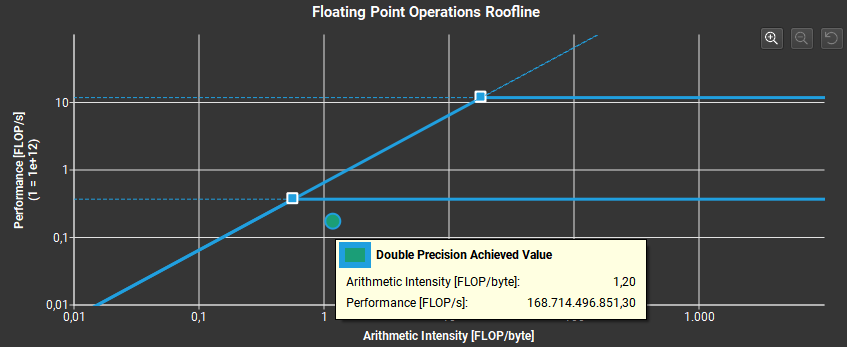
\includegraphics[width=9cm]{Images/nvidia_nsight_compute_roofline_model.png}
            \caption{ NVIDIA Nsight Compute Roofline Model }
        \end{figure}
    \end{itemize}

\end{frame}

\begin{frame}[fragile]{Memory Bandwidth IV}
    
    \begin{itemize}
        \item we observe that memory transfers from CPU to GPU and vice versa are slow
        \item Using NVIDIA's \href{https://github.com/NVIDIA/cuda-samples/tree/master/Samples/bandwidthTest}{CUDA samples}
        we are able to evaluate maximum transfer speeds in practice
        \vspace{1em}
        \begin{figure}[!H]
            \centering
            \begin{tikzpicture}[scale=0.625]
                \begin{axis}[
                    ymode=log,
                    xlabel=$\text{Size in bytes}$,
                    ylabel=$\text{Bandwidth in Gbyte/s}$,
                    xmin=1, xmax=1e6,
                    ymin=0, ymax=1000,
                    legend style={fill=none,draw=white}
                ]
            
                \addplot [magenta,mark=*,mark size=0.3pt,smooth] table [x=size,y=bandwidth,col sep=comma] {Resources/bandwidth_h_to_d.csv};
                \addlegendentry{HtoD}

                \addplot [cyan,mark=*,mark size=0.3pt,smooth] table [x=size,y=bandwidth,col sep=comma] {Resources/bandwidth_d_to_h.csv};
                \addlegendentry{DtoH}

                \addplot [orange,mark=*,mark size=0.3pt,smooth] table [x=size,y=bandwidth,col sep=comma] {Resources/bandwidth_d_to_d.csv};
                \addlegendentry{DtoD}
                \end{axis}
            \end{tikzpicture}
        \end{figure}
    \end{itemize}

\end{frame}

\begin{frame}[allowframebreaks]

    \frametitle{Bibliography}
    \bibliographystyle{acm}
    \bibliography{Bibliography/bibliography.bib}

\end{frame}


\end{document}
